\documentclass{beamer}
\usepackage{tikz}

\setbeamertemplate{navigation symbols}{}

\setbeamercolor{frametitle}{fg=orange}
\setbeamercolor{title}{fg=orange}
%\definecolor{tcolor}{RGB}{10,100,200}
\setbeamercolor{normal text}{fg=black}
%\setbeamercolor{normal text}{fg=RGB{} 
%\setbeamerfont{frametitle}{size=large}
\setbeamerfont{frametitle}{family=\rmfamily,shape=\itshape,size=\huge} 
\setbeamerfont{title}{family=\rmfamily,shape=\itshape,size=\huge} 

\usetheme{boxes}
\setbeamertemplate{background canvas}[vertical shading][bottom=white,top=blue!20]

\title{Cosmic Frontier at Brookhaven}

\begin{document}


%\frame{\titlepage}

\frame
{

    \frametitle{Dark Energy Survey (DES)}

    \fontsize{9}{0.8\baselineskip}

    \begin{columns}

        \begin{column}{0.5\textwidth}

            \begin{itemize}

                \item Imaging survey of 5000 square degrees in the southern
                    sky at CTIO.  5 optical filters, $\sim$24 mag in $i$.

                \item First light Fall 2012, survey start Aug. 31, 2013.

                \item Study Dark Energy using weak lensing, galaxy clusters,
                    large scale structure and supernovae.

                \item Erin Sheldon {\bf builder} and {\bf associate
                    member} with data rights for self, postdoc, students.

                \item Andres Plazas postdoc worked on detector characterization
                    and weak lensing of galaxy clusters (moving to JPL in Apr 2015).

            \end{itemize}

        \end{column}

        \begin{column}{0.5\textwidth}
            \includegraphics[scale=0.17]{ctio_blanco_crew_2013Oct-30-small-balance.jpg}
            \newline
            {\tiny Image: Brian Nord, FNAL}
        \end{column}

    \end{columns}

}

\frame
{
    \frametitle{Erin Sheldon DES Work}

    \begin{itemize}

        \item Full weak lensing shear pipeline developed, running on DES data.

            \begin{itemize}

                \item Same code used for galaxy fluxes, sizes and colors.

                \item With Matt Becker (Stanford/SLAC) adapting to full
                    multi-object fitting and deblending code

            \end{itemize}

        \item Science
            \begin{itemize}

                \item Shear catalogs are being used for lensing science.

                \item Galaxy catalogs being used for star-galaxy separation, beginning
                    to be used for cluster finding and photometric redshifts.

            \end{itemize}

        \item Infrastructure developed by E. Sheldon to process multi-epoch data now
            being used by QSO group; adopted by survey data management for general use.

        \item Built Crowd-sourcing ``exposure checker'', used by DES scientists
            to view images, mark bad data or processing errors, and easily
            give feedback to developers.  Developed with Peter Melchior (OSU).

    \end{itemize}

}


\frame
{

    \frametitle{Galaxy Cluster Lensing in DES}

    \fontsize{9}{0.8\baselineskip}

    \begin{columns}

        \begin{column}{0.5\textwidth}

            \begin{itemize}

                \item First results using $\sim 12,000$ galaxy clusters
                    selected from DES data

                \item Mean projected mass density constrast vs. radius

                \item Profile is dominated by Dark Matter on large scales,
                    baryonic matter on the smallest scales.

                \item Shears from pipeline developed by E. Sheldon

            \end{itemize}

        \end{column}

        \begin{column}{0.5\textwidth}
            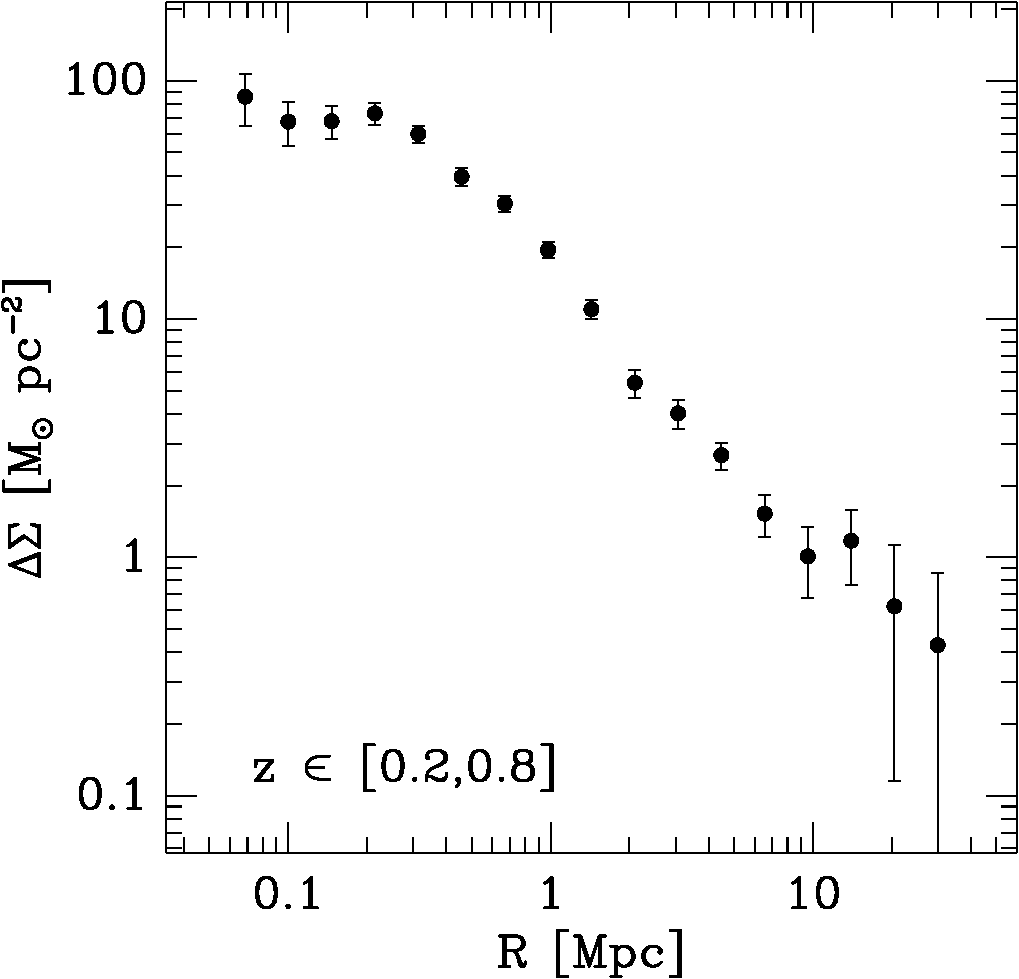
\includegraphics[scale=0.3]{run-rm008-bin-zwide-jack.pdf}
        \end{column}

    \end{columns}

}

\frame
{
    \frametitle{DES Lensing: Future Work}
    \begin{itemize}
        \item This year two papers
            \begin{itemize}
                \item Lensing studies of galaxy clusters, extend previous work
                    in the Sloan Digital Sky Survey to higher redshift
                \item Constrain dark matter distributions and halo mass function
                \item Shear methods paper
            \end{itemize}
        \item First Dark Energy studies over next couple of years as we
            process more data and improve systematics
    \end{itemize}
}

\frame
{

    \frametitle{LSST Contributions by E. Sheldon}
    \begin{itemize}
        \item Galaxy measurement code is interesting for LSST
            \begin{itemize}

                \item An order of magnitude faster than standard codes.
                \item Can fit muliple epochs and multiple bands simultaneously.  Important
                    for LSST with very large number of epochs, many bands.
            \end{itemize}

        \item I have begun working with LSST Data management team.
        \item Still in very early planning stages.

    \end{itemize}
}

\frame
{

    \frametitle{DES Detector Characterization: Tree Rings (A. Plazas)}

    show image here from Andrei
}


\frame
{

    \frametitle{DES Detector Characterization: Tree Rings (A. Plazas)}

    \begin{itemize}
        \item

            Tree-rings are features in the CCDs that occur during fabrication.
            Variations in doping produces a spurious transverse electric field,
            changing the effective location and area of each pixel

        \item In addition to intensity variations shown above, effect results
            in astrometric distortions:  problematic for lensing.

        \item The effect is now well understood and mapped out in DES images.
            We will correct in software.

        \item Paper on tree rings now published

        \item The results are now being included in the DES data
            management software (A. Plazas, G. Bernstein)

    \end{itemize}
}


\end{document}
